\chapter{Algorthmen}
\label{cha:algorithmen}
% 7 Seiten

%supervised methoden: backpropagation
%unsupervised methoden: restricted boltzmann maschines, autoencoders, sparse coding model

Fokus: viele Daten, parallele Verarbeitung, viel Rechenpower

\section{Backpropagation}

\begin{figure}
	\centering
	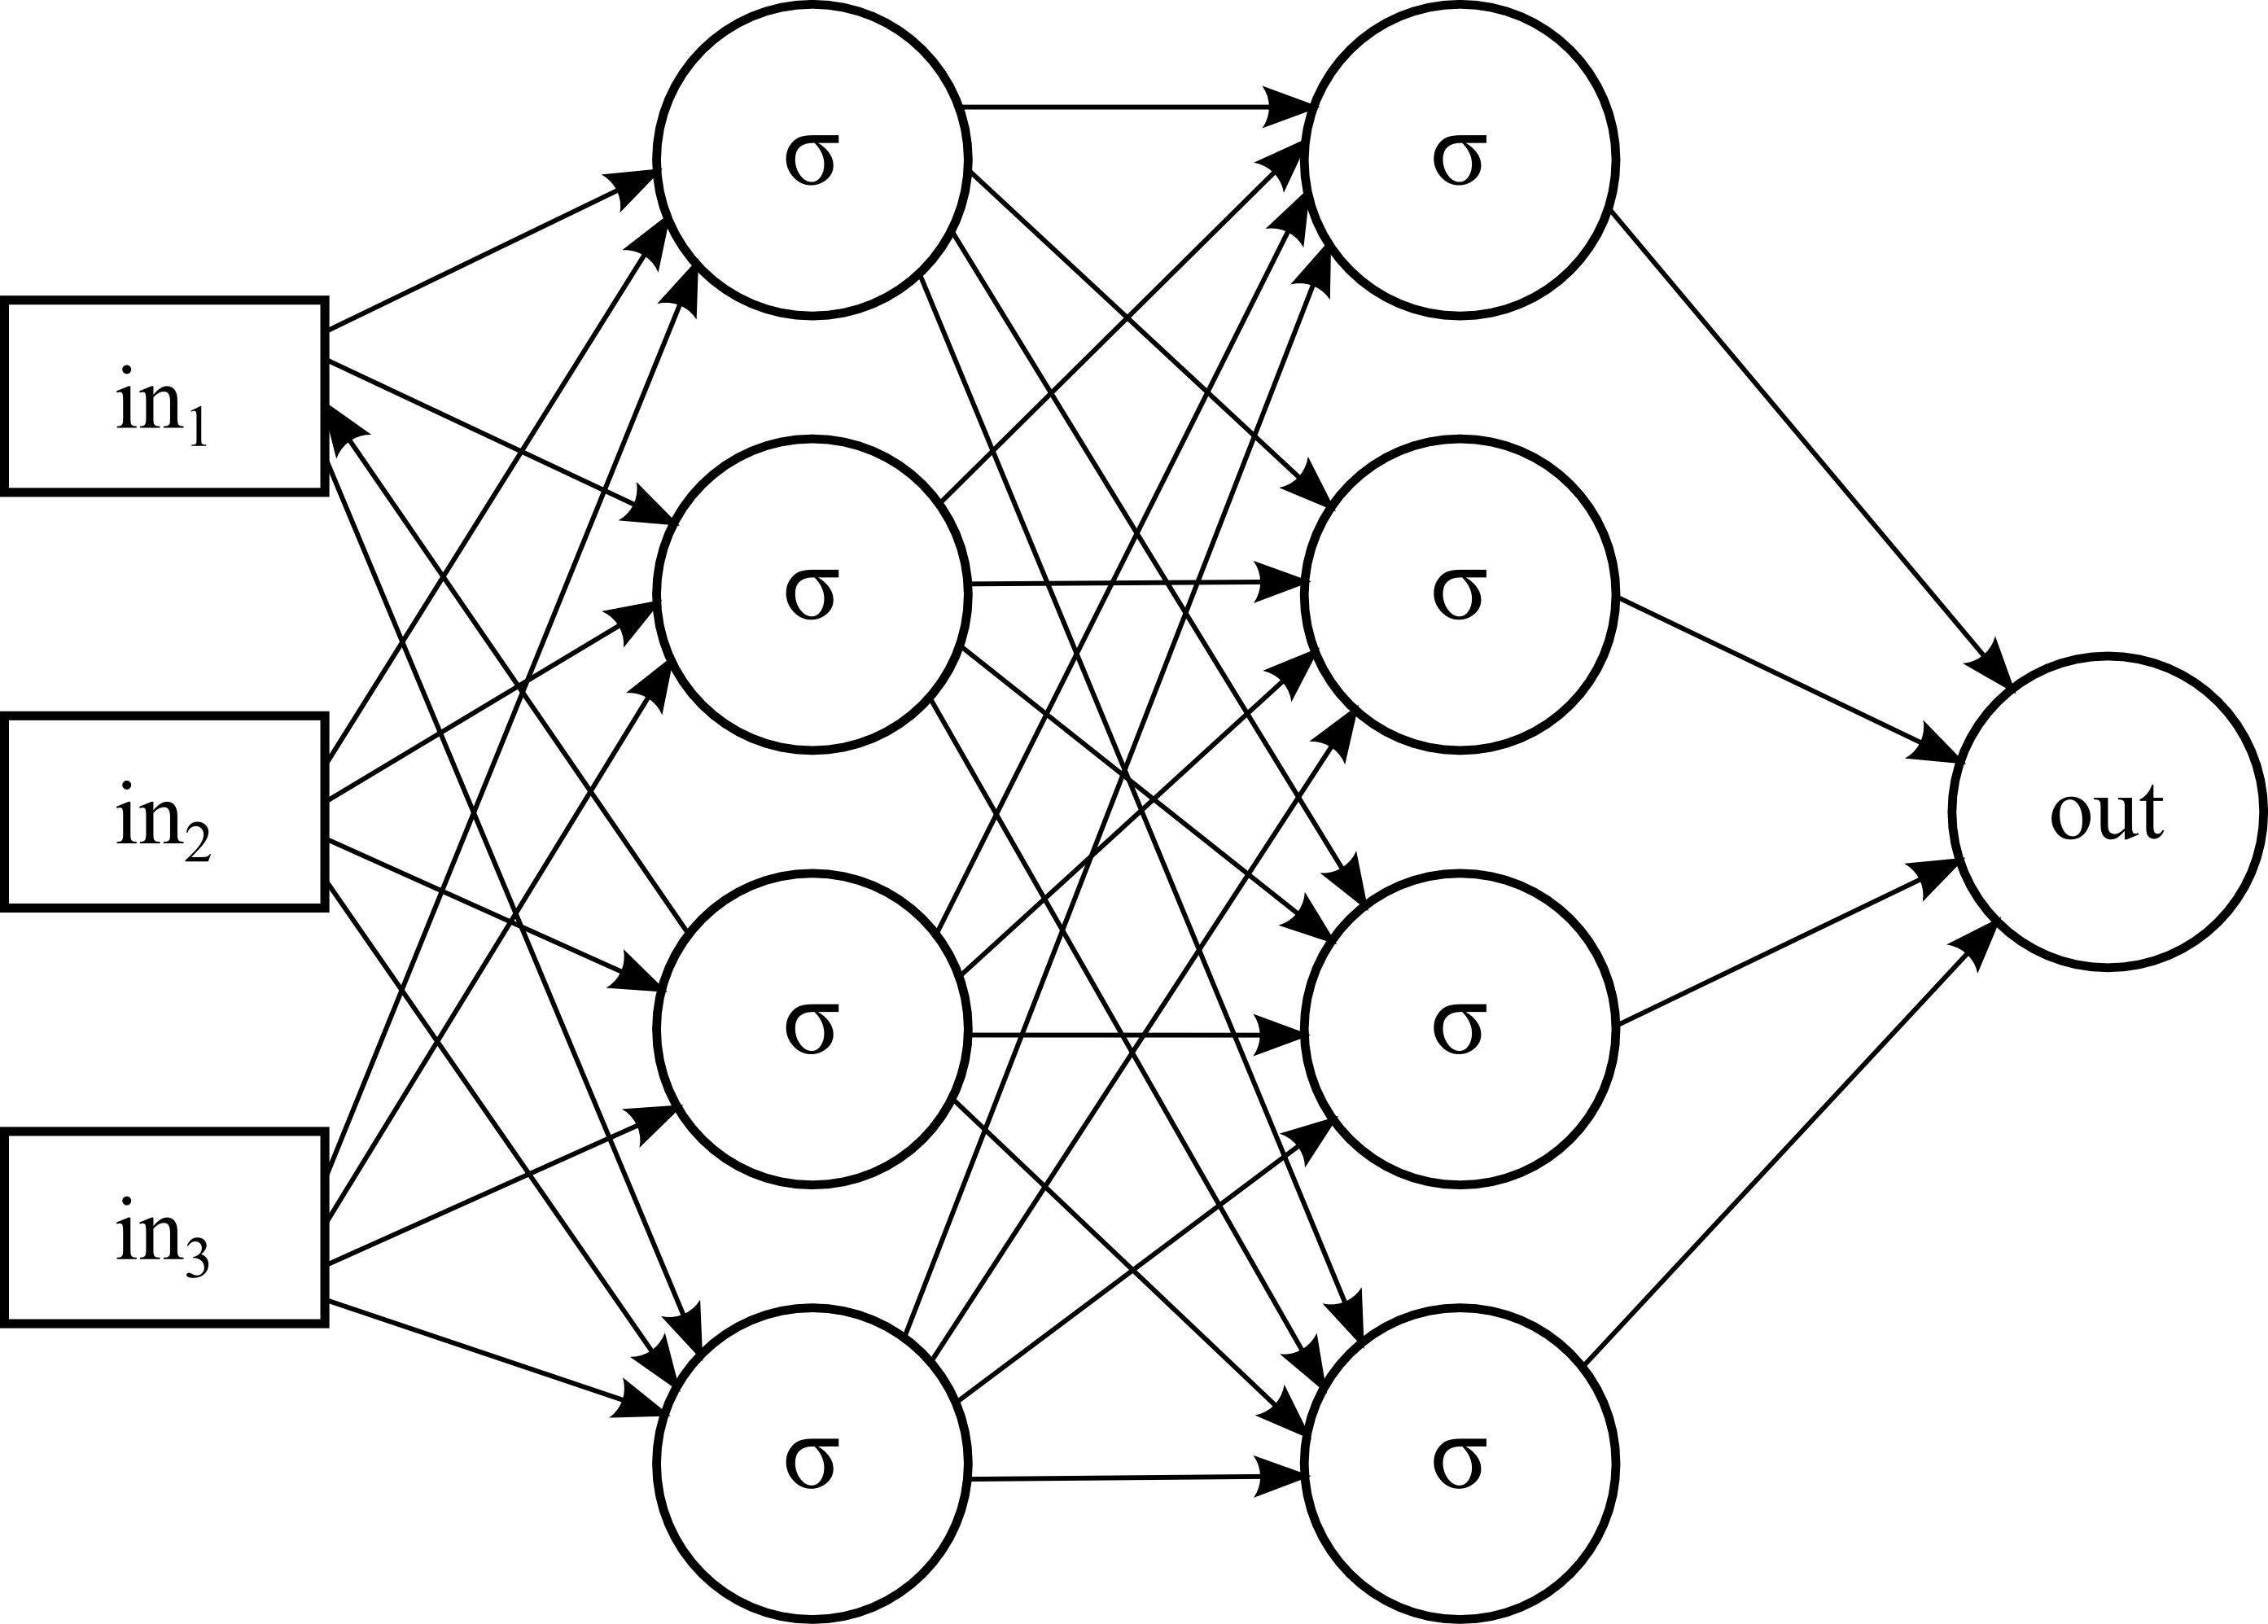
\includegraphics[scale=1]{images/net-for-bp.png}
	\caption{Ein Feedfowrward-Perzeptron}
	\label{fig:net-for-bp}
\end{figure}

Backpropagation ist ein überwachter Algorithmus zum Trainieren von vereinfachten neuronalen Netzen bei denen sich der Ausgang auf einfachem Weg berechnen werde kann, so genannten Feedforward-Perzeptrons, zu sehen in Abbildung \ref{fig:net-for-bp}. Überwacht bedeutet, dass das Netzwerk beim lernen anhand von kategorisierten Eingabedaten bestimmte Ausgabedaten zu errechnen. Der Fehler der Berechnung des Ausgangs wird beim Backpropagation-Algorithmus in die Adaptierung der Gewichte rückgeführt. Der Trainingsprozess beginnt mit zufälligen Gewichten und arbeitet in den folgenden Schritten:

\begin{enumerate}
\item Ausgang des Netzes für bestimmte Eingabedaten berechnen
\item Ausgang mit dem Sollwert vergleichen und daraus den Fehler errechnen
	$$error = \frac{1}{2}\sum_{k \in K}(out_k-target_k)^2$$
	\begin{center}\begin{tabular}{rclcrcl}
		$target$ & \dots & Fehler, der später Einfluss in die Gewichte nimmt\\
		$out$ & \dots & Wert den der Ausgang erreicht hat\\
		$target$ & \dots & Wert den der Ausgang erreichen sollte\\ 
		$K$ & \dots & Anzahl der Neuronen in der Ausgangsschicht\\
	\end{tabular}\end{center}
\item Gewichte je nach Größe des Fehlers anpassen
\end{enumerate}

Diese Schritte werden wiederholt, bis die Gewichte so angepasst wurden, das Eingabedaten möglichst gut klassifiziert werden können. Die Anpassung der Gewichte errechnet sich im wesentlichen anhand der Gradienten der Fehler und Gewichte. Zudem nimmt Schicht, vor der sich das jeweilige Gewicht befindet, Einfluss.

\begin{figure}
	\centering
	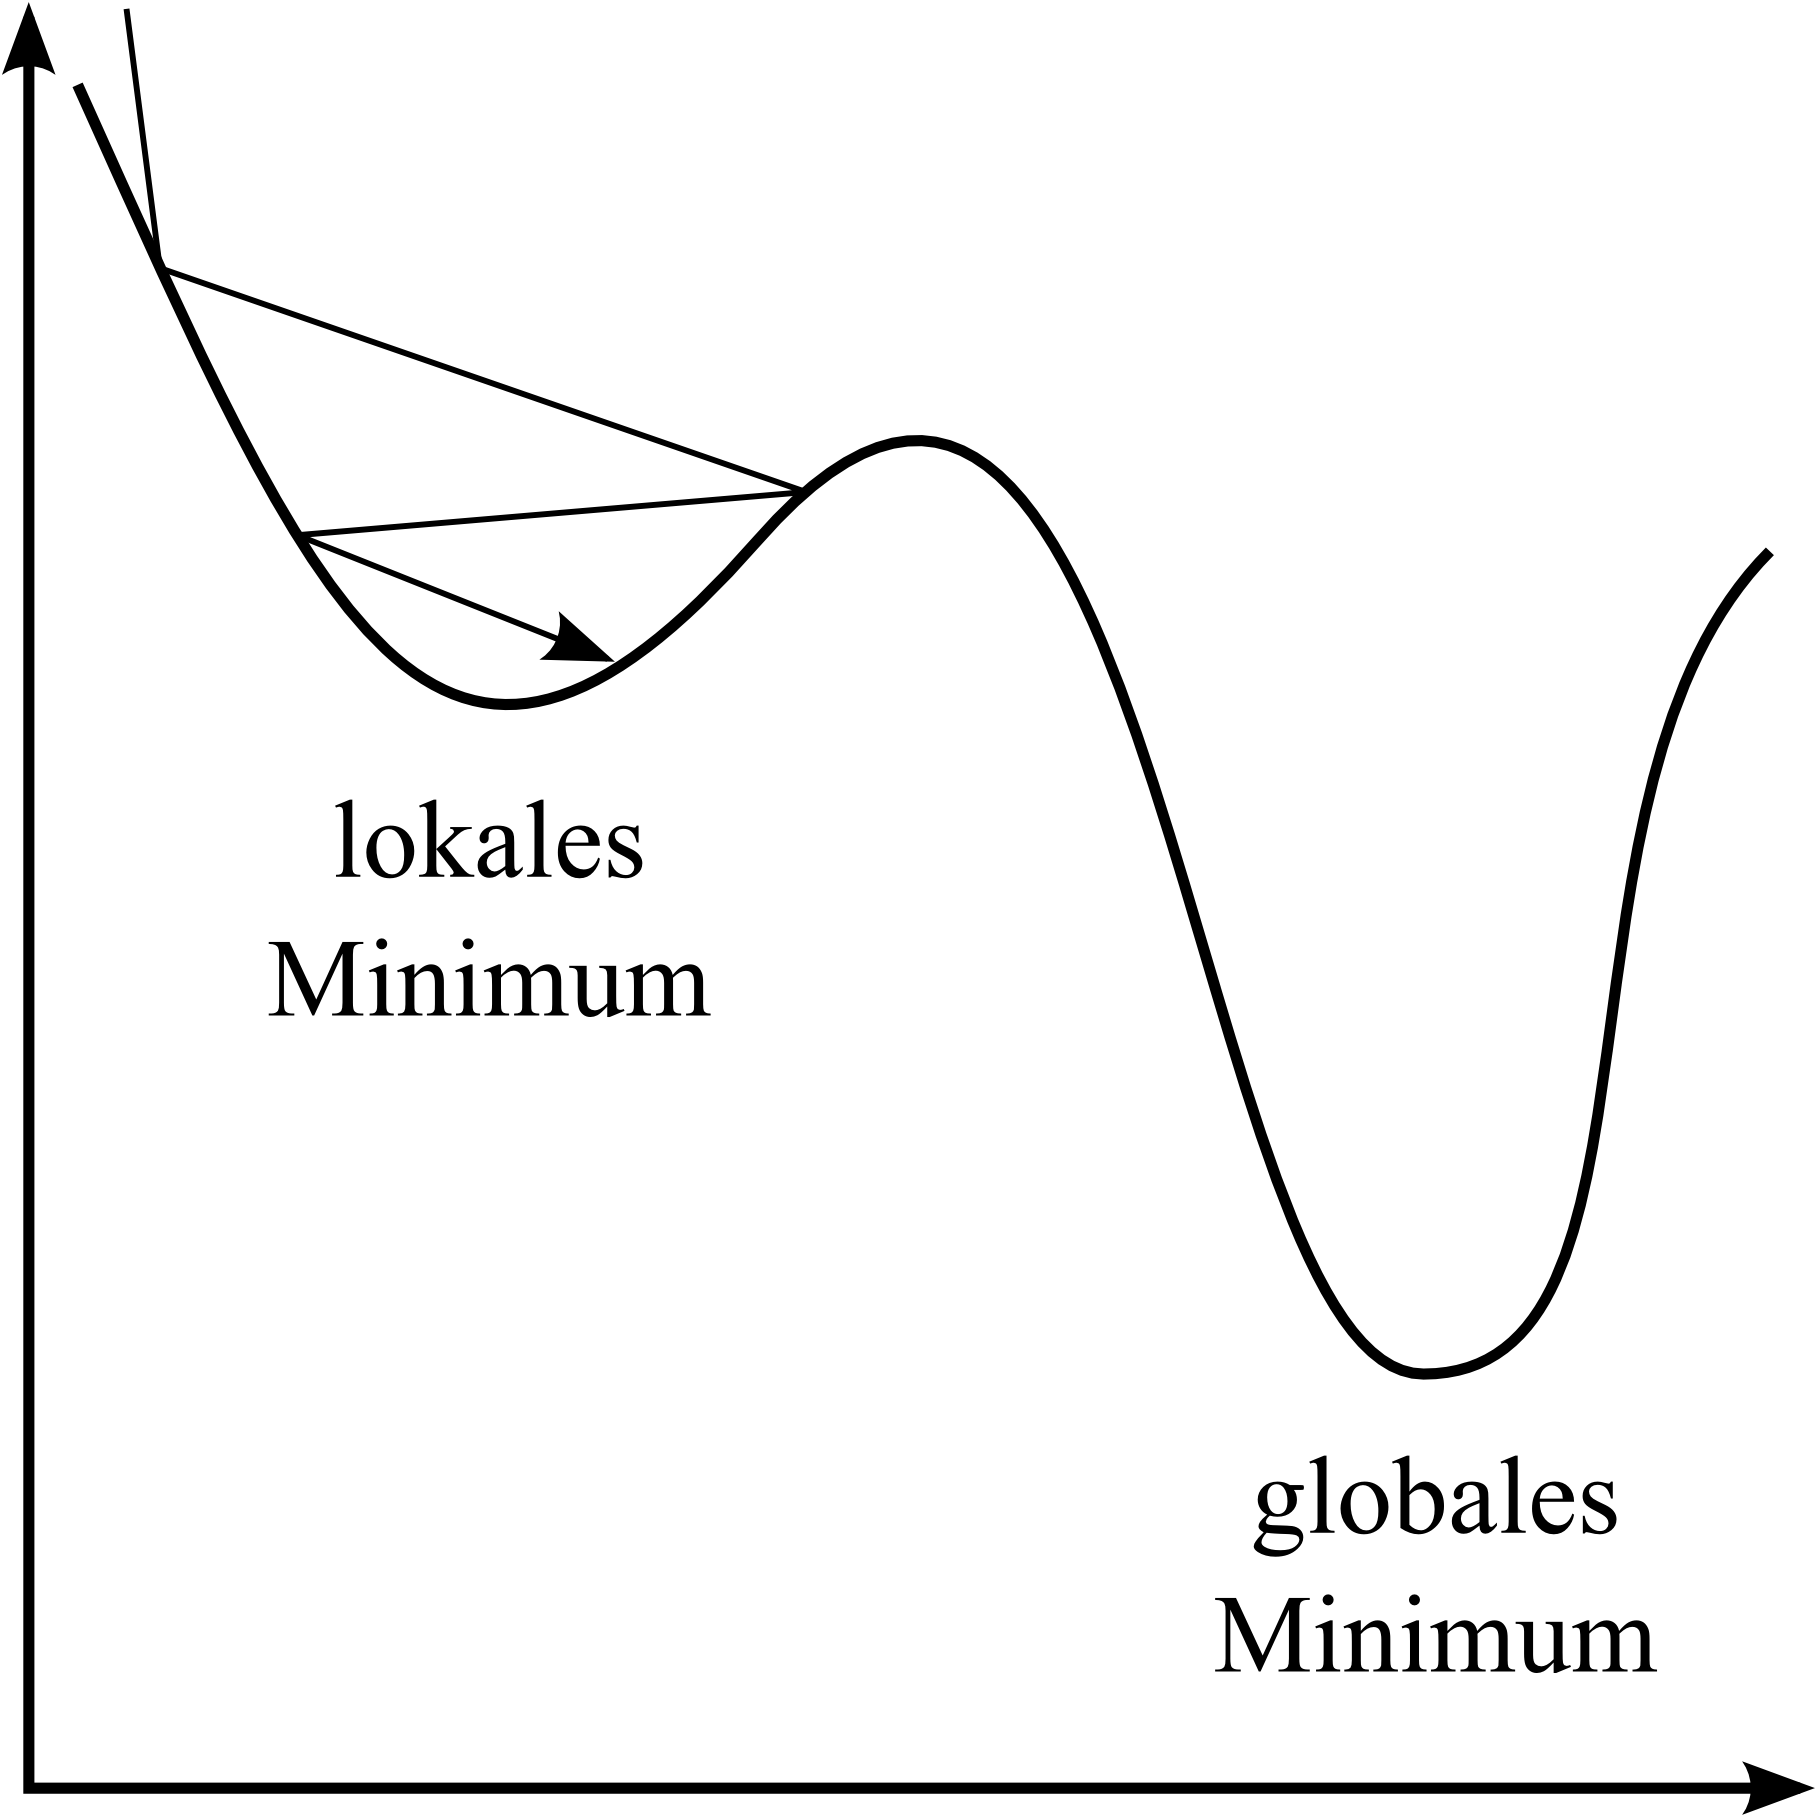
\includegraphics[scale=1]{images/lokales-minimum.png}
	\caption{Lokales Minimum}
	\label{fig:local-min}
\end{figure}

Wie der Name des Alogorithmus bereits verrät, wird der Fehler dabei im wesentlichen über eine mathematische Funktion in die Gewichte zurückgeführt. Diese Rückführung bringt das Problem von lokalen Minima mit sich. Wird die Änderung des Fehlers geringer, so wird auch die Anpassung geringer. Befindet man sich auf dem Weg in ein lokales Optimum, wie in Abbildung \ref{fig:local-min} zu sehen, so kann dieses sehr weit weg von dem globalen Optimum sein. Ist das Optimum entsprechend groß, so ist die Wahrscheinlichkeit, dass der Algorithmus in diesem Optimum hängen bleibt groß. Abhilfe können hier Verfahren wie der Bergsteigeralgorithmus oder zusätzliche Zufallswerte bei der Berechnung der Gewichte schaffen.

Der Algorithmus trainiert vordefinierte Ein- und Ausgabedaten mit dem Ziel für ähnliche Daten ähnliche Ergebnisse zu liefern. Trainiert man das Netz zu intensiv mit diesen Daten, so lernt es genau nur diese Trainingsdaten. Dies hat zur Folge, dass das Netz im späteren Betrieb schlechtere Ergebnisse liefert als hätte man es weniger lange trainiert.

\section{Resctricted Boltzmann Maschines}

\begin{figure}
	\centering
	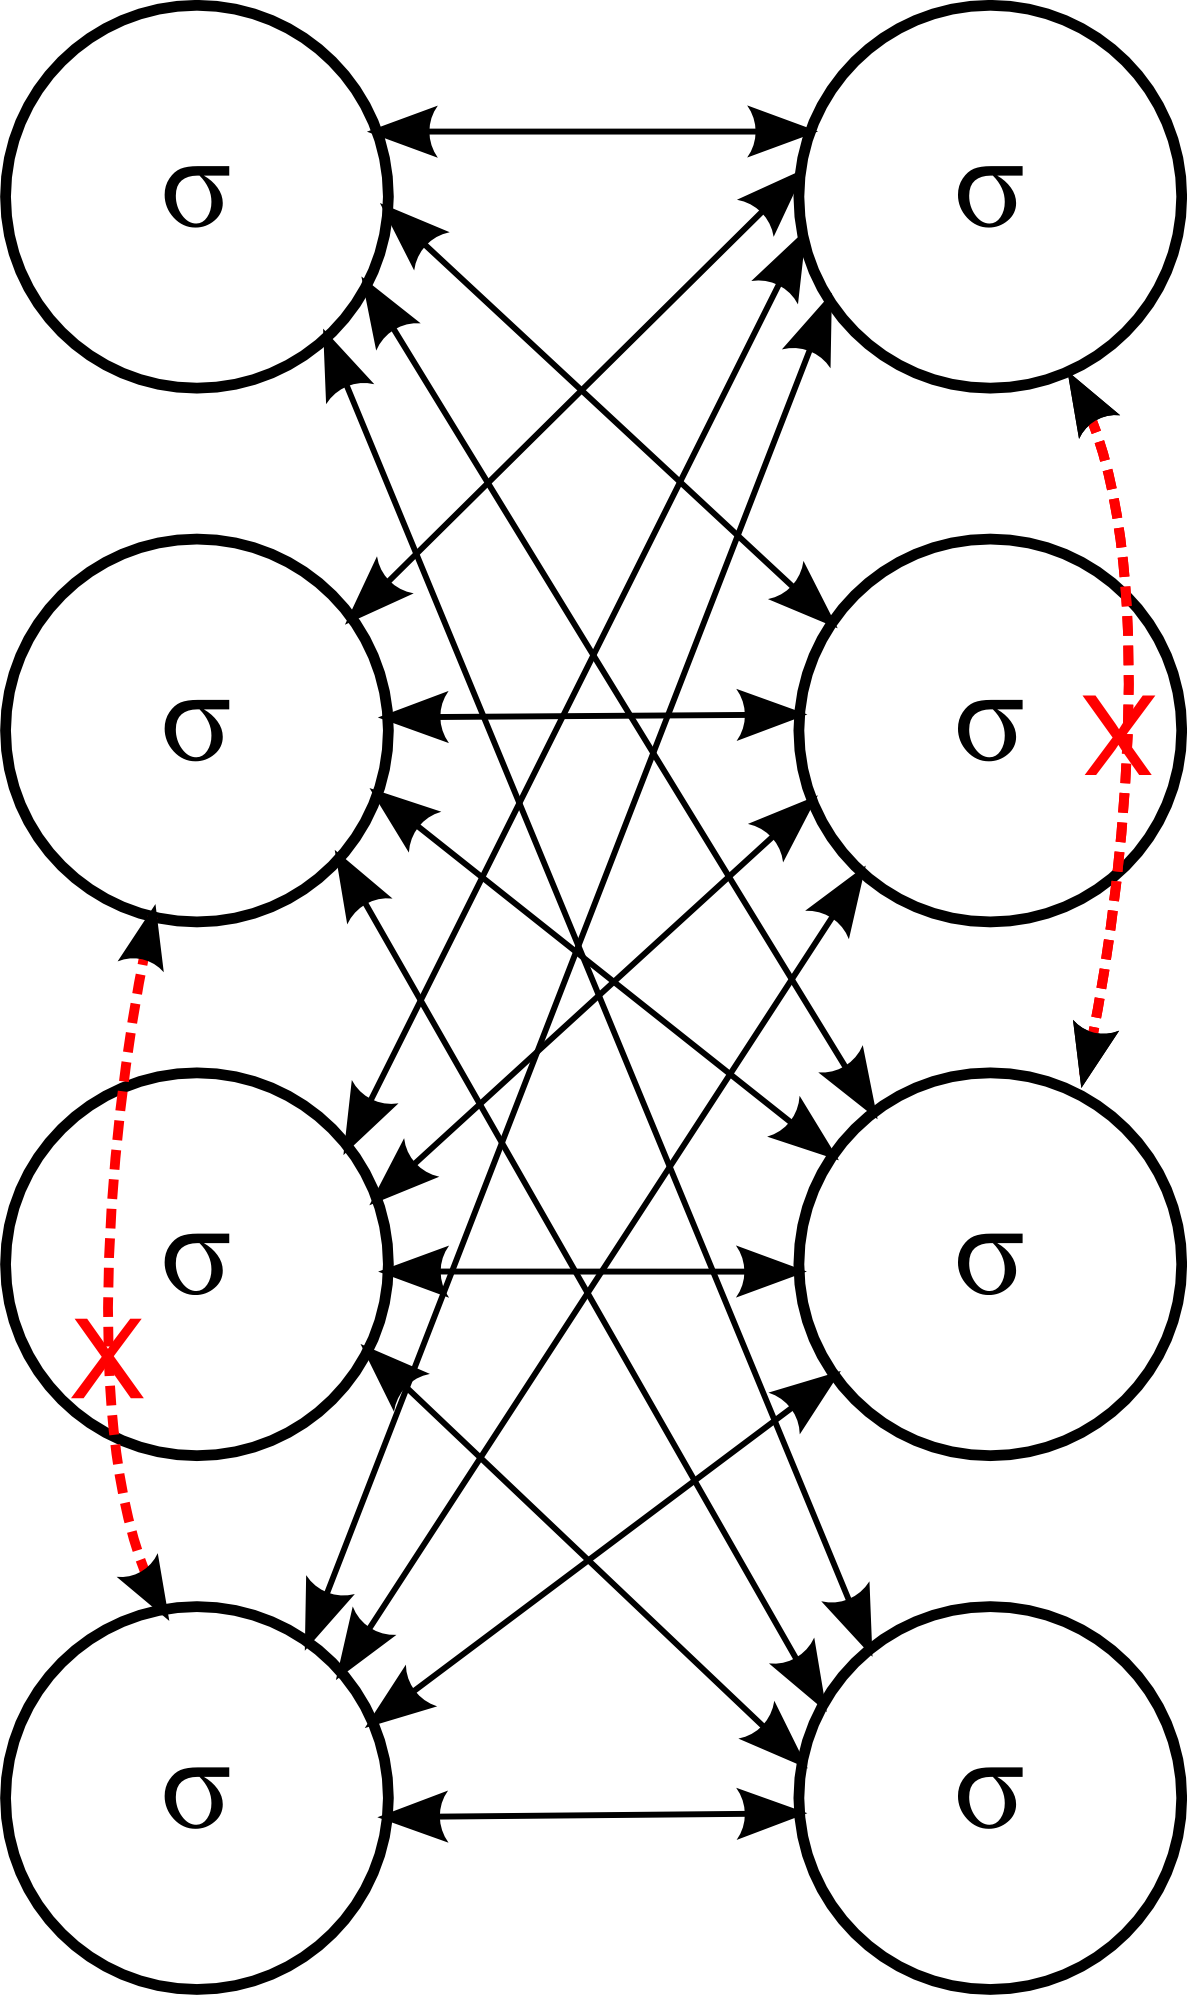
\includegraphics[scale=1]{images/rbm.png}
	\caption{Eine Restricted-Boltzmann-Maschine}
	\label{fig:rbm}
\end{figure}

Uneingeschränkte Neuronale-Netze sind schwierig und aufwendig zu trainieren. Restricted-Boltzmann-Maschines, im weiteren auch als RBMs bezeichnet, sind eingeschränkte neuronale Netzwerke. Wie in Abbildung \ref{fig:rbm} dargestellt, existieren hierbei nur Verbindungen zwischen aneinander liegenden Schichten. Das Modell erlaubt keine Verbindungen von Neuronen zu sich selbst und alle Verbindungen müssen gleichermaßen in beide Richtungen gehen. So lassen sich unter Festlegung der Werte einer Schicht direkt auf die nächste versteckte Schicht weiter gerechnet werden. RBMs arbeiten in der Regel mit bool'schen Werten, lassen sich durch Erweiterung aber auch mit anderen Zahlenräumen verwenden.

RMBs wurden bereits 1986 von Paul Smolensky \todo{ref} unter dem Namen Harmonium erfunden, fanden jedoch erst 1998, rund 10 Jahre später, durch die Entwicklung von effizienten Lernalgorithmen durch Geoffrey Hinton Anwendung.

Zum trainieren von RMBs existieren verschiedene Algorithmen, die meist auf dem Prinzip beruhen, die Gewichte so anzupassen, das das hin und her Rechen zwischen zwei Schichten wieder die Ausgangsdaten ergibt. Im folgenden wird der Algorithmus von Geoffrey Hinton \todo{reference}, der zugleich als der erste effizienten Lernalgorithmus für RMBs gesehen wird, erklärt. 

\subsection{Grundgedanke}

\begin{figure}%
\centering
\subfloat[Versteckte Schicht berechen]{\begin{minipage}{0.33\textwidth}\centering%
	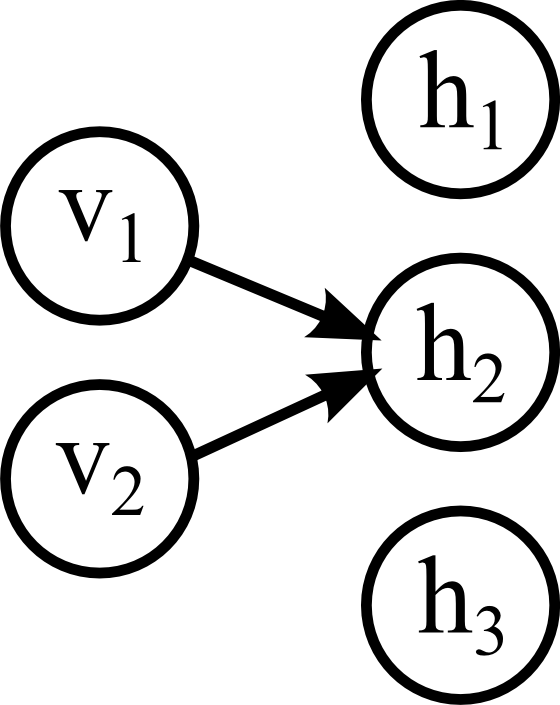
\includegraphics[scale=1]{images/rbm-step1.png}\end{minipage}}
\subfloat[Von der versteckten Schicht zurück rechnen]{\begin{minipage}{0.33\textwidth}\centering%
	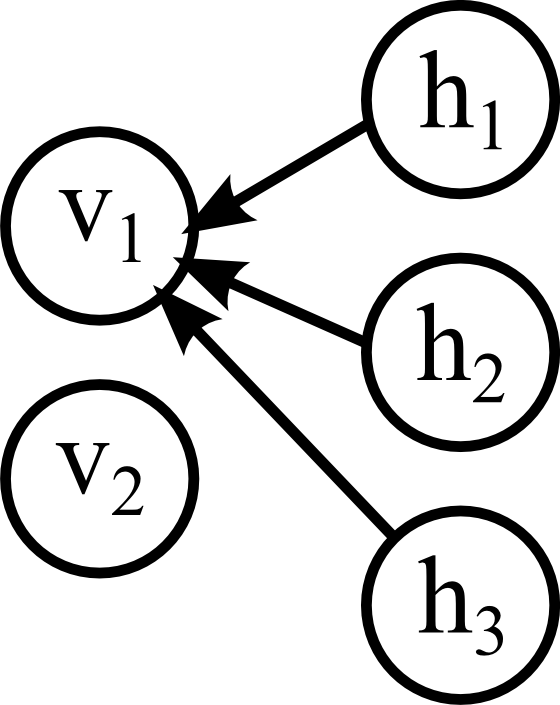
\includegraphics[scale=1]{images/rbm-step2.png}\end{minipage}}
\subfloat[Erneut die versteckte Schicht berechnen]{\begin{minipage}{0.33\textwidth}\centering%
	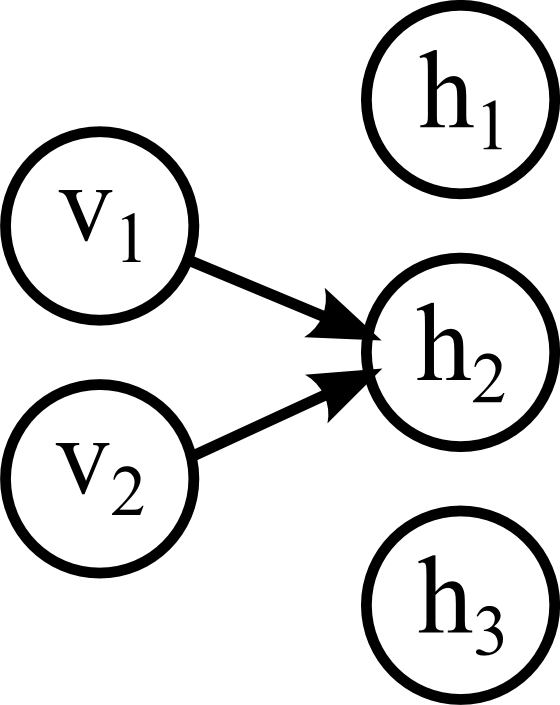
\includegraphics[scale=1]{images/rbm-step3.png}\end{minipage}}
\caption{Drei Berechnungsschritte zum Lernen von RBMs.}
\label{fig:rbm-steps}
\end{figure}

Sind die Werte einer Schicht fixiert, so kann einfach auf die nächste versteckte Schicht weiter gerechnet. Zu beginn werden wird ein Trainingsdatenset an die Eingänge angelegt und die folgenden Operationen, wie auch in Abbildung \ref{fig:rbm-steps} zu sehen, wiederholt ausgeführt:

\begin{enumerate}
\item Wahrscheinlichkeit $p$ für die versteckten Neuronen $h_j$ anhand der sichtbaren Neuronen $v_i$ und der Gewichte $w_{ij}$ berechnen $$p(h_j=1) = \frac{1}{1+e^{-(b_j+\sum_{i}(v_i*w_{ij}))}}$$
\item Werte für die versteckte Schicht aus dem Mittelwert der Wahrscheinlichkeiten berechnen
\item Gradientenmatrix $<v_ih_j>$ über das dyadische Produkt errechnen $$<v_ih_j> = v*y^T$$
\item Ausgehend von den errechneten versteckten Neuronen, zurück auf die sichtbare Schicht rechnen
\end{enumerate}

Wiederholt man die in der Liste angeführten Schritte sehr oft, so pendeln sich für die Neuronen Werte ein, die im wesentlichen vom Modell und den den Wahrscheinlichkeiten abhängen, jedoch sehr wenig mit den Eingangsdaten zu tun haben. Anhand der Gradientenmatrix des letzten Durchlaufes lässt sich jedoch eine Distanz zum gewünschten Modell herausfinden und so können die Gewichte wie folgt angepasst werden:
$$\Delta\omega_{ij} = \varepsilon (<v_ih_j>^0 -  <v_ih_j>^\infty)$$

Diese Art der Berechnung lieferte sehr gute Modelle. Durch die vielen Iterationen benötigt der Algorithmus sehr viel Rechenzeit und ist daher nicht praxistauglich. Zudem ist es schwierig festzustellen, wie viele Iterationen bis zum Einpendeln notwendig sind.

\subsection{Abkürzung}

Der oben genannte Algorithmus lässt sich in seiner Komplexität erheblich reduzieren, in dem die versteckte Schicht lediglich zwei mal berechnet wird. Geoffrey Hinton hat mit der Vereinfachung gezeigt, dass es möglich ist, bereits mit dem Vergleich der ersten und zweiten Gradientenmatrix möglich ist gute Ergebnisse zu erzielen. Diese Methode wird \emph{Contrastive Divergence} genannt.

Die Regel zur Anpassung der Gewichte lautet dann:
$$\Delta\omega_{ij} = \varepsilon (<v_ih_j>^0 -  <v_ih_j>^1)$$

\subsection{Begründung}

Der Grundgedanke von \emph{Contrastive Divergence} ist, dass das Modell mit Zufallsgewichten weg von den Eingabedaten, hin zu Daten die ihm besser gefallen, wandert. Wenn man erkennt wo hin das Modell die Daten ändert, kann man die Gewichte so adaptieren, dass dem Modell die Eingabedaten am besten gefallen.

\subsection{Eignung}

Das Modell besitzt nicht genügend Neuronen um alle Eingabedaten zu speichert und muss daher, um die Eingabedaten tatsächlich reproduzieren zu können, etwas aus den Eingabedaten lernen. Es eignet sich daher, um aussagekräftige Merkmale aus unkategorisierten Daten zu extrahieren.

\section{Deep Autoencoders}

\begin{figure}
	\centering
	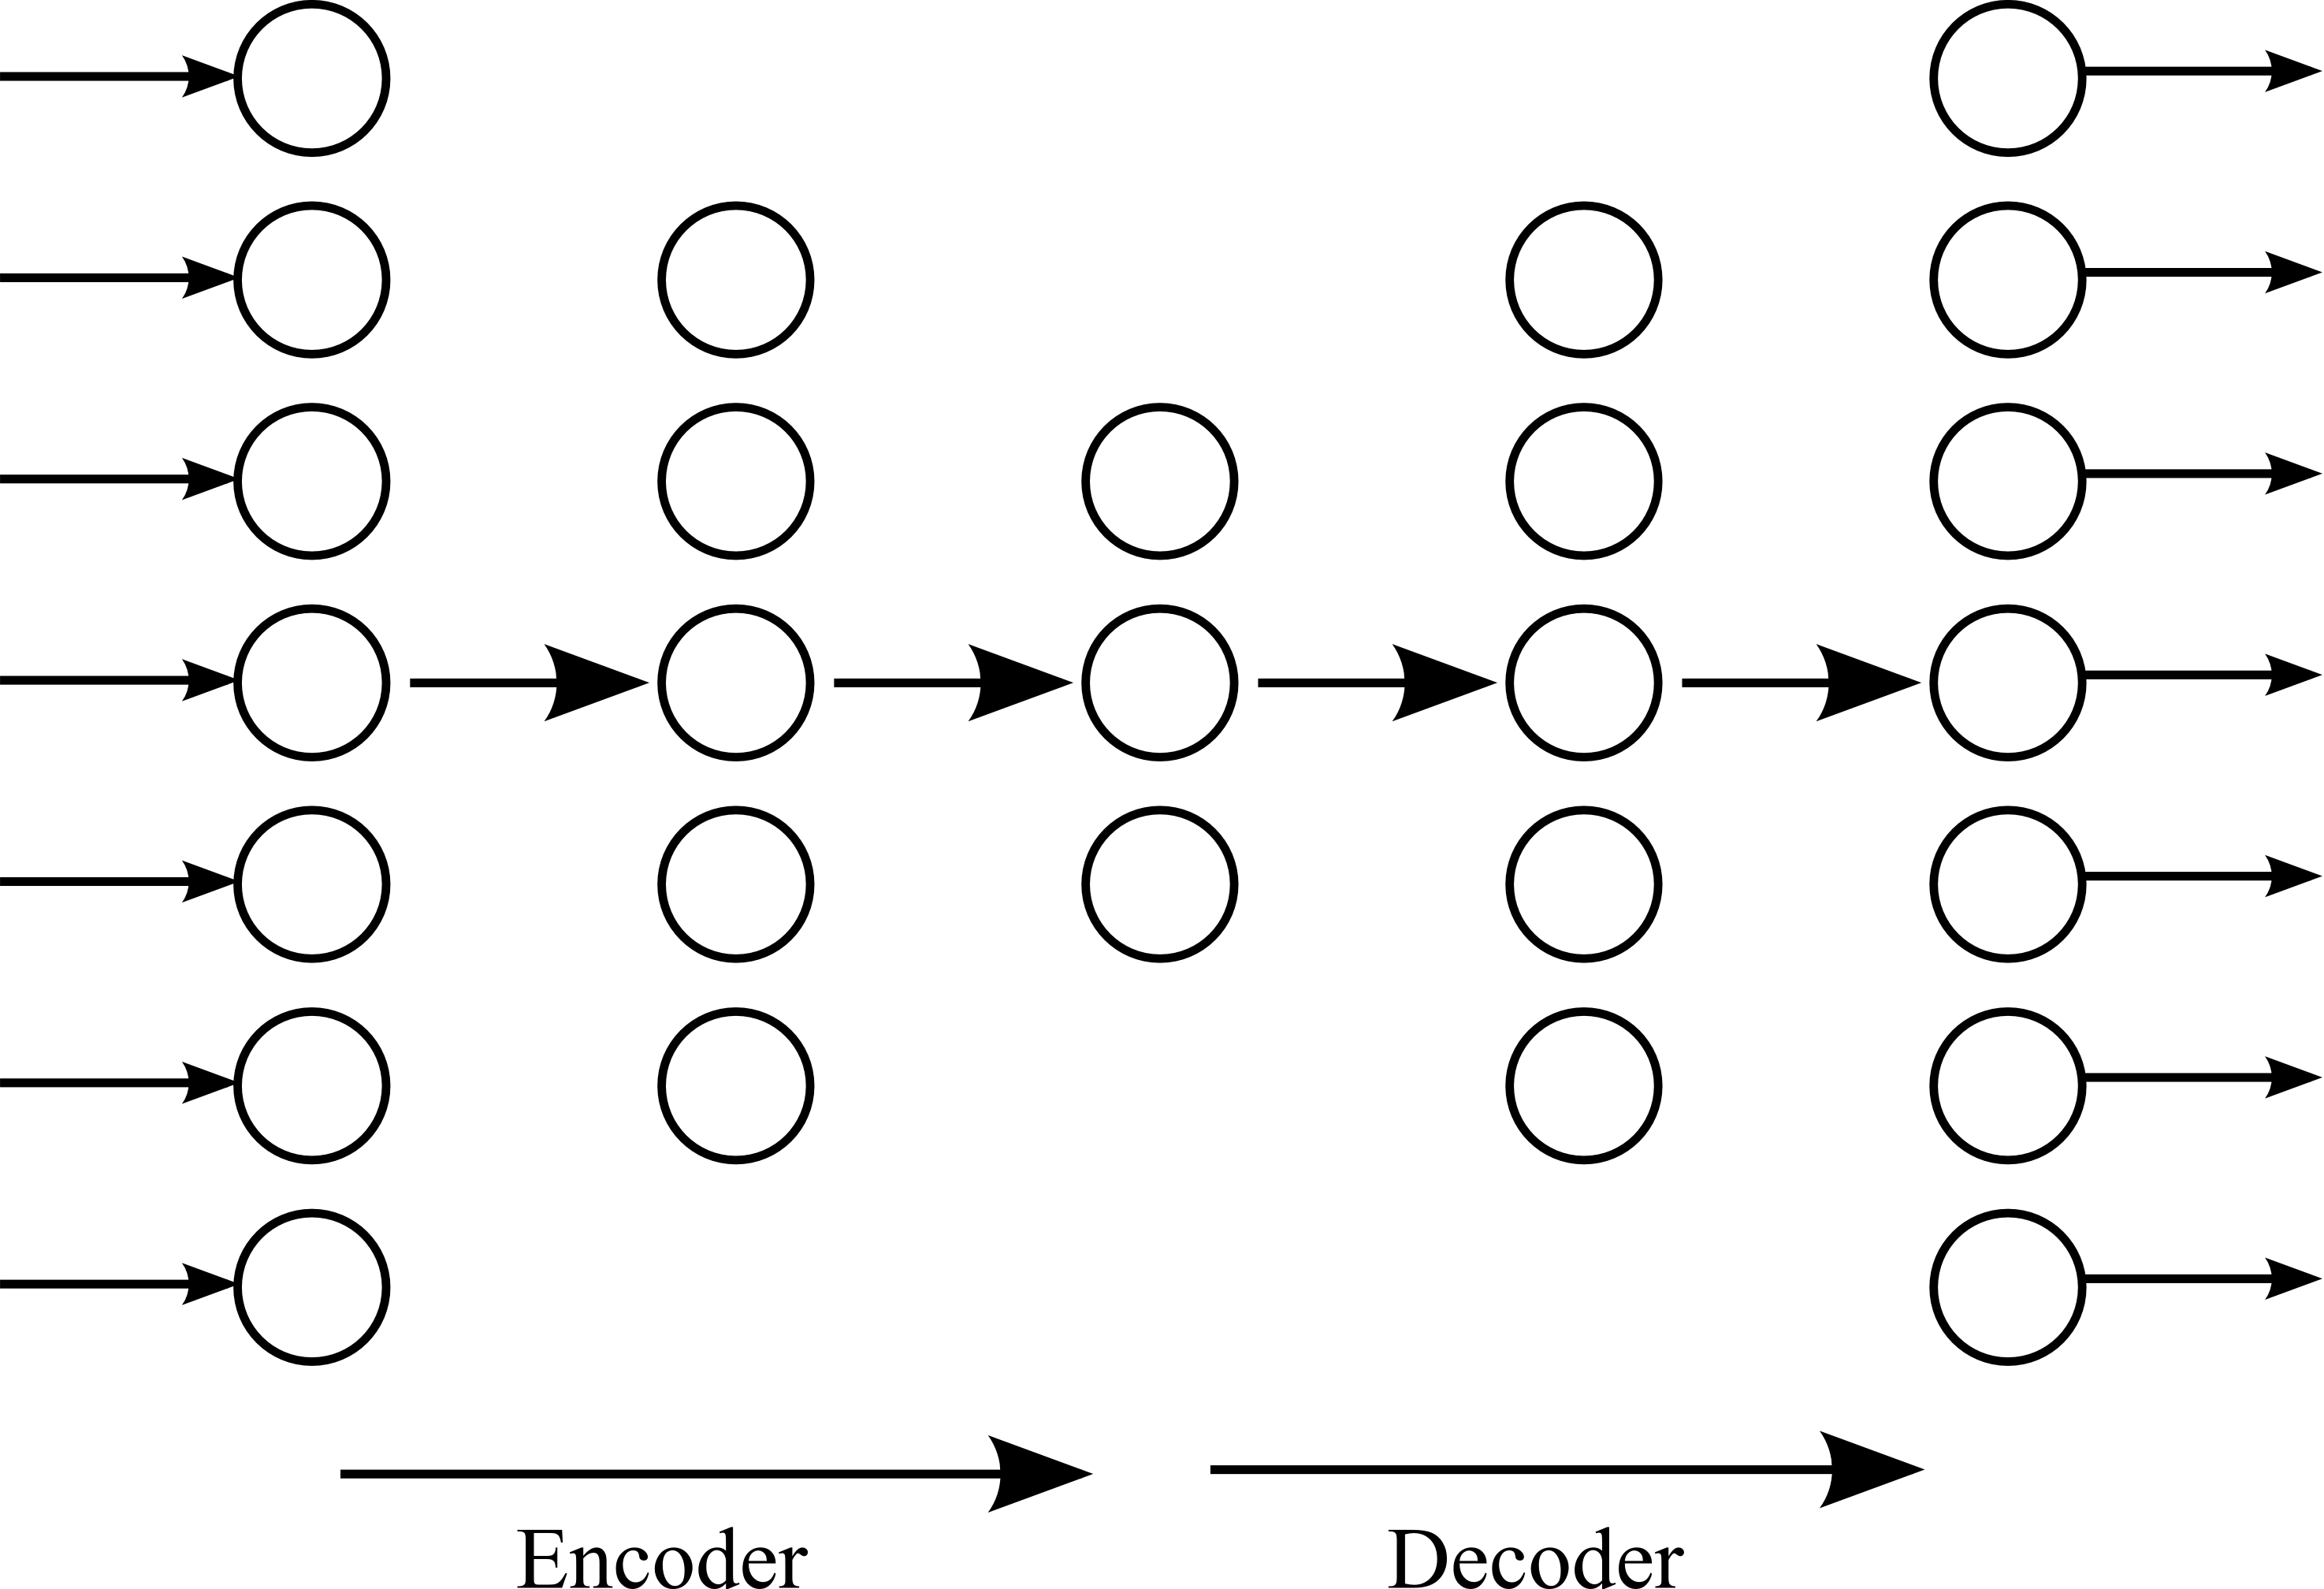
\includegraphics[scale=1]{images/autoencoder.png}
	\caption{Deep Autoencoder}
	\label{fig:autoencoder}
\end{figure}

Deep Autoencoder sind neuronale Netze aus mehreren Schichten, die sich in zwei wesentliche Teile trennen lassen. Im ersten Teil, dem Encoder, sinkt die Anzahl der Neuronen mit jeder Schicht, während sie im zweiten Teil, dem Decoder wieder Steigt, bis am Ende wieder die Anzahl der Eingangsparameter erreicht ist. Abbildung \ref{fig:autoencoder} zeigt ein solches Netz. Im inneren hat das Netz weniger Neuronen und somit Speichermöglichkeit als Eingangsparameter. Es wird versucht das Netz so zu trainieren, dass es am Ausgang die gleichen Daten berechnet wie am Eingang angelegt entstehen. Gelingt das Training, so muss das Netz Merkmale etwas aus den Daten gelernt haben.

Richtig trainiert, komprimiert das Netz die Daten also. So wäre es zum Beispiel möglich Bilder durch das Netz zu schicken, die kleinste Schicht zu speichern und jederzeit über den Decoder wiederherzustellen. Für Bilder, Ton und Videos gibt es einige Kompressionsalgorithmen die sehr fein abgestimmt die Charakteristik menschlicher Organe berücksichtigt und daher in der Regel wesentlich bessere Ergebnisse liefern. Dennoch demonstriert das Beispiel, dass damit unter Umständen erheblich Speicher und Verarbeitungsleistung gespaart werden kann.

Deep Autoencoder liefern sehr vergleichbare Ergebnisse und werden daher gerne als Benchmark für Deep Learning-Algorithmen verwendet. Deep Autoencoders tendieren zu Unteranpassung (eng. underfitting), da nicht genügend Neuronen verfügbar sind um alle Möglichkeiten abzubilden. Eine einfache und effektive Variante ein solches Netz zu trainieren ist es, jeweils zwei Layer separat als restricted Boltzmann Maschine anzusehen.

Lernt man solche Algorithmen mit mit Bildern und visualisiert die entstandenen Gewichte, so erkennt man, dass solche Algorithmen in erster Instanz meist Kanten und Farbintensitäten in Bildern finden. In der zweiten Schicht findet man einfache Kombinationen dieser Elemente und ab der dritten Schicht werden meist schon sehr brauchbare Neuronen zur vollständigen Objekterkennung ausgebildet.

\section{Faltungscodierte neurale Netze}
% als grundlage

Faltungskodierte neuronale Netze (eng. Convolutional Neural Networks) sind neuronale Netze die zur Reduktion der Gewichte in einzelne Teile zerteilt sind. Bei den bisher angeführten Netzen wurden jeweils alle Neuronen einer Schicht mit jedem Neuron der nächsten Schicht verbunden. Der Gedanke bei faltungskodierten Netzten geht man davon aus, dass weit voneinander entfernte Neuronen kaum etwas miteinander zu tun haben, während nahe aneinander liegende Neuronen Zusammenhänge besitzen. Es werden daher Gruppen über aneinander liegende Neuronen gebildet, die untereinander in die nächste Schicht verknüpft sind. Wie am Beispiel eines Bildes gut erkennbar, ist es gut möglich, dass ein Merkmal nicht genau in eine dieser Gruppen passt. Es werden daher viele überlappende Gruppen gebildet.

\begin{figure}
	\centering
	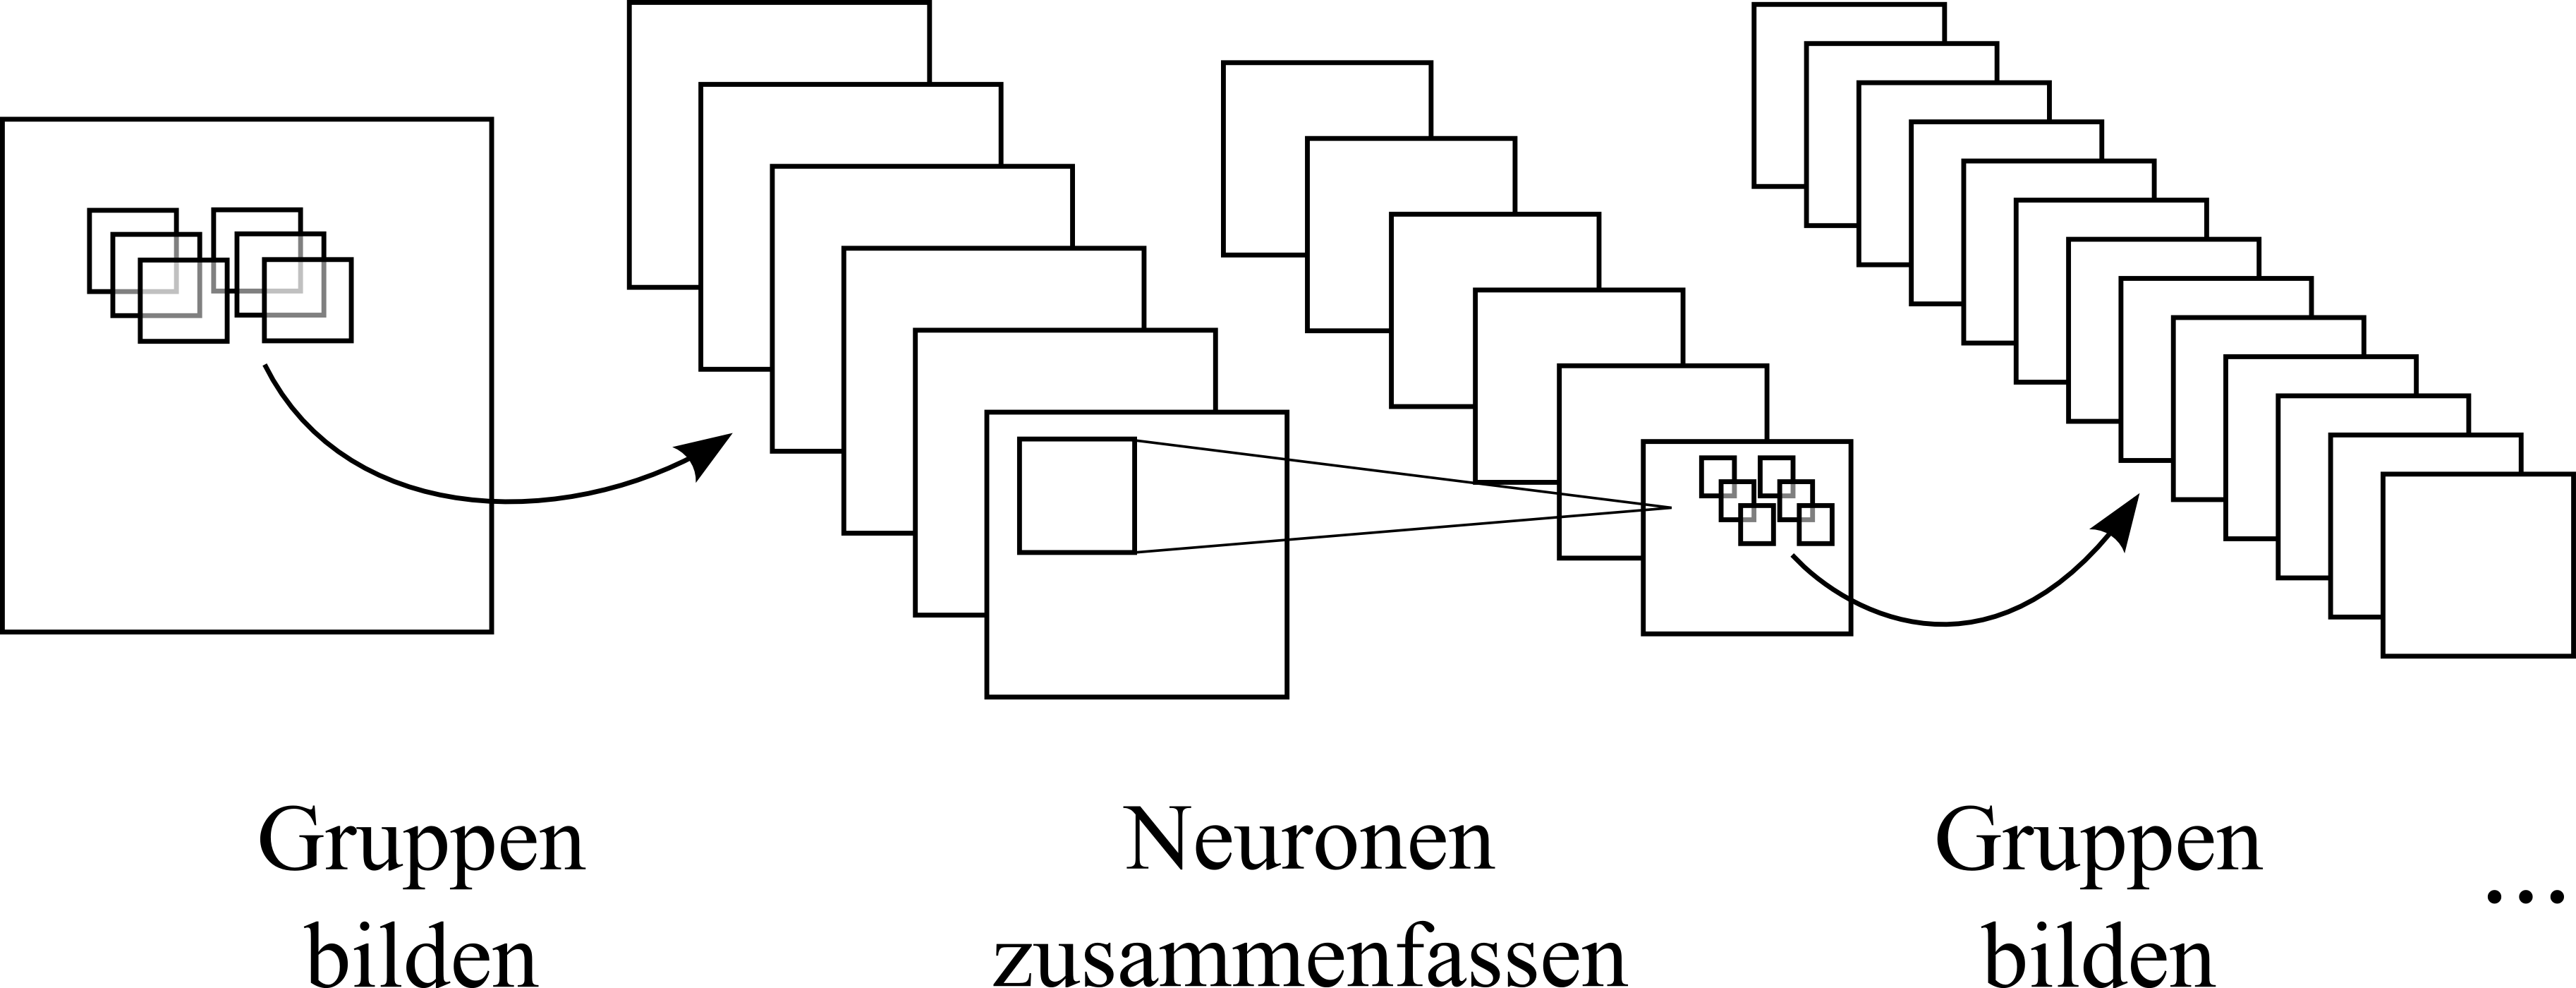
\includegraphics[scale=1]{images/convolution.png}
	\caption{Faltungscodiertes neuronales Netz}
	\label{fig:convolution}
\end{figure}

Im nächsten Schritt gibt es eine zusammenfassende Funktion, die die Ergebnisse aneinander liegender Werte für die nächste Schicht mit einer mathematischen Funktion zusammenfasst. Diese Funktion könnte in einer Schicht zum Beispiel die Rotation eines Bildes ignorieren in dem es Kanten in mehrere Richtungen zusammenfasst. Ein faltungskodiertes neuronales Netz wiederholt genau diesen zwei Komponenten, die überlappende Gruppierung von Neuronen so wie das zusammenfassen von Neuronen auf jeder Schicht. Abbildung \ref{fig:convolution} zeigt ein solches Netz.

Dieser Typ von Netzwerk ist bereits 1980 \todo{paper Kunihiko fukushima} bekannt, wurde in den folgenden Jahrzehnten optimiert und erlebte einen Aufschwung durch parallelisierte Berechnung auf einer GPU \todo{Dan Ciresan}. Nach weiteren Optimierungen in den vergangen Jahren wurde ein solches Netzwerk unter anderem für ein Projekt von Google \todo{google paper finden} eingesetzt, das nicht zuletzt das so genannte face-neuron ausprägte.

\section{Sparse coding}

Sparse coding ist ein Algorithmus zum trainieren eines neuronalen Netzes mit dem Ansatz möglichst aussagekräftige Merkmale zu finden. Anders als beim Deep Autoencoder wird hier nicht nur berücksichtigt wie gut das Ergebnis wiederhergestellt werden konnte, sondern auch wie eindeutig das Ergebnis war. Ziel ist es an möglichst vielen stellen im Ausgangsvektor 0er zu haben und dennoch sehr gute Ergebnisse zu finden. Der Fehler setzt sich aus diesen beiden Faktoren zusammen und wie folgt berechnet:

$$min\frac{1}{T}\sum_{t=1}^{T}min\frac{1}{2}|x^{(t)}-D*h^{(t)}|+\lambda|h^{(t)}_1|$$
\begin{center}\begin{tabular}{rclcrcl}
	$x^{(t)}$ & \dots & Eingangswert\\
	$h^{(t)}$ & \dots & Ausgangswert\\
	$D$ & \dots & Anzahl der Ausgänge\\
	$\lambda$ & \dots & Steuert wie stark sich die 0er im Ausgangsvektor auswirken\\ 
\end{tabular}\end{center}

Die zwei Bedingungen widersprechen sich teilweise und können über $\lambda$ balanciert werden. Die Berechnung der Gewichte für die versteckten Schichten ist beim Sparse Coding wesentlich aufwendiger als bei Deep Autoencodern, da es sich hier um ein Optimierungsproblem und nicht nur um eine lineare Funktion handelt.